\chapter{Kuinka järjestelmä hajautetaan?}
\begin{it}
	Kirjoita tähän yleistä tietoa tästä kappaleesta. Tietona ulos tulee lukijalle mitä tässä kappaleessa käsitellään kokonaisuudessaan. Tämän voisi kijoittaa viimeisenä.
\end{it}
Aikaisemmin käsiteltiin erilaisia hajautuksen paradigmoja ja kuinka osapuolet voivat kommunikoida hajautetussa järjestelmässä. Tässä kappaleessa analysoidaan näitä paradigmoja ja arvoidaan mitkä sopisivat tässä työssä suunniteltavan ohjelmistokomponentin tarkoituksiin. Lisäksi käsitellään avointa AMQP-kommunikointistandardia (engl. Advanced Message Queing Protocol), joka mahdollistaa erilaisten hajautusparadigmojen toteutuksen osapuolten välillä. AMQP:stä käsitellään sen toiminnallisuutta ja kuinka se sopii tämän työn tarpeisiin.

% TODO: Kirjoita tämä vastaamaan muuta tekstiä kun muut kappaleet ovat valmiit.


\section{Arkkitehtuurin analyysi}
\label{ch:architecture-analysis}
IEC 61850 -standardi määrittää, että viestit IED-laitteelta tulevat julkaisija-tilaaja-pa\-ra\-dig\-man mukaisesti. Viestit tilataan IED-laitteelta olevilta RCB-luokkien instansseilta. RCB-instanssi on kytketty laitteella olevaan datajoukkoon, jonka tiedoista ollaan kiinnostuneita. Rajoituksena standardi asetti, että RCB-instanssi täytyy tilaajan varata ja yksi RCB-instanssi voi palvella vai yhtä tilaajaa kerrallaan. RCB-instansseja IED-laitteissa on rajallinen määrä yhtä datajoukkoa kohti ja näitä voidaan myös käyttää aseman sisäiseen toimintaan. Tässä työssä käsitellyssä IED-laitteessa yhteen datajoukkoon oli esimerkiksi määritetty viisi eri RCB-instanssia. Seurauksena on, että kyseisen datajoukon voi tilata vain viisi saman aikaista tilaajaa. Lisäksi tässä työssä testattu IED-laite rajoitti avoimet yhteydet viiteen. Tästä ylimeneviä yhteyksiä ei avattu ja IED-laite palautti standardin mukaisen negatiivisen vastauksen.

Vaatimuksissa määriteltiin että IED-laitteen tieto täytyy saada jaettua järjetelmän muiden komponenttien kanssa. Työn tekohetkellä komponentteja järjestelmässä oli kaksi. Mittaustiedon näyttämiseen ja tilatiedon tarkkailuun. Vaatimuksissa kuitenkin määriteltiin, että toteutuksessa haluttiin varautua tulevaisuuden varalle komponenttien suhteen. Eli tilanteeseen jossa niitä olisi enemmän kuin kaksi ja niiden määrä voisi vaihtua tilaamisen aloitusten välillä. 

Edelle mainituista IED-laitteen rajoituksista ja työlle asetetuista vaatimuksista voidaan tehdä johtopäätöksiä hajautuksen arkkitehtuurin suhteen. Samalle IED-laitteelle avattujen yhteyksien määrä halutaan pitää pienenä. Tämän lisäksi varattujen RCB-instanssien määrä jokaista datajoukkoa kohti halutaan myös pitää pienenä. Nämä sen takia, koska halutaan mahdollisimman vähän varata aseman resursseja sen muulta käytöltä. Lisäksi järjestelmän IED-laitteelta vaatimat resurssit halutaan pitää ennalta määrättynä lukuna. Tämä helpottaa aseman insinöörin suunnittelutyötä, koska hän voi ottaa luvut huomioon IED-laitteiden konfiguroinnissa.

Edellä mainittuun tilanteeseen ratkaisuna voisi ajatella, että järjestelmän yksittäiset komponentit tilaisivat niiden tarvitsemat tiedot suoraan IED-laitteelta. Ongelmana tässä kuitenkin on aikaisemmin mainittu yhteyksien määrän rajoitus IED-laitteelle ja niiden määrä haluttiin minimoida ja pitää vakiona. Lisäksi viestit tilataan ja palautetaan komponentille MMS-protokollamäärityksien mukaisesti. Seurauksena on, että jokainen komponentti joutuu käsittelemään MMS-protokollan binääridataa itse tai kirjaston avulla. Viestin muoto olisi parempi olla ymmärrettävämpi. Näin viestin lukeminen eri tekniikoilla olisi helpompaa. Tämä asetettiin ohjelmiston vaatimuksissa ja oli myös yksi kohta työlle asetetuista tutkimuskysymksistä.

Ratkaisuna edellä mainittuun tilanteeseen on kommunikoinnin epäsuoruuden lisääminen. Samoin menee myös kuuluisa lainaus henkilöltä David Wheeler \cite[s.~290]{beautiful-code}:
\begin{quote}
	All problems in computer science can be solved by another level of indirection.
\end{quote}
Epäsuoruutta saadaan aikaan toteuttamalla erillinen ohjelmistokomponentti IED-laitteen ja muiden järjestelmän komponenttien väliin. Tätä komponenttia voisi kutsua myös nimellä \emph{väliohjelmisto} (engl. \emph{middleware}). Väliohjelmisto tilaisi viestit IED-laitteelta ja halutuilta RCB-instansseilta. Samalla komponentti muokkaisi saapuvat viestit parempaan muotoon, joka olisi helpompi muiden järjestelmän komponenttien lukea. Väliohjelmiston avulla yhteyksien määrä IED-laitetta kohti saadaan yhteen. Tämän avulla myös saadaan minimoitua varattujen RCB-instanssien määrä datajoukkoa kohti yhteen. Tuloksena on vakiomäärät yhteyksiä ja RCB-istansseja datajoukkoa kohti jotka ovat helpompi ennustaa ja konfiguroida etukäteen tarpeiden mukaan.

Vaatimuksissa mainittiin myös, että muu järjestelmä ohjaa viestien tilauksen aloittamista ja lopettamista. Väliohjelmistoa on mahdollista muun järjestelmän ohjata tarvittavin tilauksien mukaan. Tietysti tieto tilauksesta täytyy myös saada järjestelmän muille komponenteille. Väliohjelmisto ja epäsuoruus myös helpottavat viestien puskuroinnin toteuttamista komponenteille, joka myös oli vaatimuksena. Ilman epäsuoruutta, jokaisen komponentin pitäisi toteuttaa oma sisäinen puskuri viestien vastaanottamiseen.

Tässä kappaleessa analysoitiin IEC 61850 -standardin asettamia rajoja ja ohjelmistolle asetettuja vaatimuksia. Näistä analysoitiin mikä olisi toimiva ratkaisu tässä tilanteessa järjestelmän hajauttamiseen korkealla tasolla. Tuloksena järjestelmään päätettiin lisätä epäsuoruutta toteuttamalla väliohjelmisto IED-laitteen ja järjestelmän muiden komponenttien väliin. Tuloksena jää vielä miettiä mitkä kommunikointiparadigmat toteuttavat väliohjelmiston ja komponenttien vaatimukset? Mihin muotoon MMS-tason viesti väliohjelmistossa pitäisi muuttaa jakoa varten? Mitkä ovat väliohjelmiston ja muiden komponenttien väliset liitoksien vahvuudet? Kuinka viestien puskurointi väliohjelmiston avulla toteutetaan?

% TODO: Lisää tähän kuva selventämään kahta vaihtoehtoa jossa komponentit tilaavat viestit ied-laitteelta ja missä väliohjelmisto tilaa viestit sen sijaan. Lukijalle helpottamaan ymmärrystä mistä puhutaan.


\section{Osapuolten liitoksien analyysi}
Aikaisemmin kappaleessa \ref{ch:liitokset} käsiteltiin hajautetun järjestelmän osapuolten välisiä liitoksia. Erilaiset liitoksien luokittelut esiteltiin taulukossa \ref{tab:communication-models}. Lisäksi hajautetussa järjestelmässä kommunikointi osapuolten välillä voi olla suoraan tai epäsuoraa. Aikaisemmin kappaleessa \ref{ch:architecture-analysis} päädyttiin lisämään epäsuoruutta IED-laitteen ja järjestelmän muiden komponenttien väliin.

IED-laitteen ja viestien tilaajan välinen kommunikointi on suoraa ja se ei tapahtu välikäden kautta. Lisäksi osapuolten välillä on vahva tila- ja aikaliitos. Tilaliitos tulee kun kummatkin osapuolet tietävät toistensa identiteetin (IP-osoitteen). Aikaliitoksessa osapuolien täytyy olla olemassa samaan aikaan. Tilaajan täytyy olla ottamassa viesti vastaan kun IED-laite viestin lähettää ja IED-laitteen täytyy olla olemassa kun tilaus tehdään. Kaikki edellemainitut tulevat IEC 61850 -standardin määrityksien seurauksena ja näihin ei työn puitteissa voi vaikuttaa.

Työn aloitushetkellä järjestelmässä oli kaksi tietoa tarvitsevaa komponenttia. Vaatimusten mukaan haluttiin varautua tulevaisuuten, jossa niitä voisi olla enemmänkin. Tästä seurauksena väliohjelmiston ja muiden järjestelmän komponenttien välinen suhde on yksi-moneen. Vaatimuksena oli, että tietoa tarvitsevien komponenttien määrä pystyisi muuttumaan tilauksien välillä. Toteuttamalla suora kommunikointi väliohjelmiston ja järjestelmän muiden komponenttien väliin. Väliohjelmiston tarvitsee tietää muiden komponenttien olemassaolosta ja kenelle viestit täytyy ohjata. Tämä lisäisi osapuolten välistä riippuvuutta ja vähentäisi toteutuksen joustavuutta. Ratkaisuna on lisätä epäsuoruutta väliohjelmiston ja muiden komponenttien väliin välikädellä. Välikäsi vähentää osapuolten välistä riippuvuutta ja lisää toteutuksen joustavuutta. Se myös auttaa toteuttamaan asetettuja vaatimuksia, kuten viestien puskurointia ja uuden viestin ilmoitusta. Vaatimuksena oli, että IED-laitteelta tulevaa tietoa pitäisi pystyä jakamaan komponenteille IED-laitteen perusteella. Välikäden tuoma epäsuoruus auttaa myös tämän vaatimuksen toteuttamisessa. Tällä vastuu väliohjelmistolta viestien jakamisesta saadaan siirrettyä välikäden vastuulle.

Väliohjelmiston ja muiden komponenttien välille edellä mainitun perusteella halutaan heikko tilaliitos. Väliohjelmiston ei tarvitse tietää järjestelmän muiden komponenttien identiteettiä ja tämä parantaa toteutuksen joustavuutta. Aikaliitos asetettujen vaatimuksien perusteella pystyisi olemaan vahva tai heikko. Kuitenkin muu järjestelmä ohjaa tilauksen aloittamista, jolloin muutkin komponentit tietävät asiasta. Tämä vaatimus poistaa tarpeen heikolle aikaliitokselle.

Tässä kappaleessa analysoitiin hajautetussa järjestelmässä osapuolten välisi liitoksien vahvuutta. IEC 61850 -standardi asettaa rajoitteet IED-laitteen ja väliohjelmiston välille, joihin ei voida vaikuttaa. Väliohjelmiston ja muiden komponenttien väliin päädyttiin toteuttamaan epäsuora kommunikointi joustavuuden ja vaatimusten takia. Samojen osapuolten väliin halutiin toteuttaa heikko tilaliitos ja vahva aikaliitos. Kysymyksenä jää miettiä millä hajautuksen paradigmoilla välikäsi pitäisi toteuttaa, jotta halutut ominaisuudet saadaan toteutettua? Näitä olivat viestien puskurointi, ilmoitukset uuden viestin saapuessa ja viestien jakaminen komponenteille IED-laitteen mukaan.

% TODO: Lisää tähän kuva joka jatkaa edellistä kuvaa ja mitä tuli lisää tämän kappaleen pohjalta.


\section{Sopivien paradigmojen analyysi}
\begin{it}
	Kirjoita tähän analyysia aikaisemmin käsitellyistä paradigmoista ja peilaa niitä ohjelmistolle asetettuihin vaatimuksiin. Tietona sisään tulee vaatimukset mitkä asetettiin aikaisemmin ja kaikki käsitellyt paradigmat. Näistä tulee ulos selvästi miksi tarvittiin viestijonoa ja julkaisija-tilaaja-paradigmaa.
\end{it}
Hajautettussa järjestelmässä osapuolet voivat kommunikoida monen eri tavoin. Aikaisemmin esiteltiin tässä työssä suunniteltavan ohjelmistokomponentin vaatimukset mitä sen pitäisi pystyä täyttämään. Tässä kappaleessa analysoidaan hajautuksen eri paradigmoja ja verrataan niitä asetettuihin vaatimuksiin. Tarkoituksena on analysoida mitkä paradigmat sopisivat tämän työn toteutukseen parhaiten.




\subsection{Prosessien välinen kommunikointi}


\subsection{Etäkutsu}


\subsection{Tilaaja-julkaisija}


\subsection{Viestijono}


\section{Tekniikan valinta}
\begin{it}
	Kirjoita tähän tekniikan valinnasta. Miksi valittiin AMQP-standardi. Voisi sanoa pari sanaa myös muista standardeista kuten MQTT. Tietona ulos tulisi kuinka AMQP sopii tähän toteutukseen ja se tarjoaa kaikki vaaditut ominaisuudet.
\end{it}


\section{Advanced Message Queuing Protocol (AMQP)}
\label{ch:amqp-theory}
Työssä toteutettu ohjelmisto tilasi viestit IED-laitteen RCB-instansseilta. Viestit tilattiin verkon yli aseman ulkopuolelle. Ohjelma prosessoi IEC 61850 -standardin mukaiset viestit ja lähetti ne eteenpäin välittäjälle (engl. message broker). Välittäjä on verkossa oleva erillinen palvelin, mistä muut ohjelmat pystyvät tilaamaan viestejä tarpeidensa mukaan. Kuvassa \ref{fig:implemented-system-communication} on esitetty lopullisen toteutuksen tietoliikenne eri osapuolten välillä. Tässä työssä toteutettu ohjelmisto on merkitty kuvaan katkoviivalla. Toteutuksessa oli kyse julkaisija-tilaaja-arkkitehtuurimallista (engl. publish-subscribe pattern), jossa toteutettu komponentti oli tilaaja IED-laitteelle ja julkaisija välityspalvelimelle. Järjestelmän muut komponentit olivat tilaajia välityspalvelimelle. Tässä osuudessa perehdytään viestien välittäjän teoriaan, ja mitä siitä täytyy tietää ohjelmistokehityksen kannalta.

\begin{figure}[ht!]
	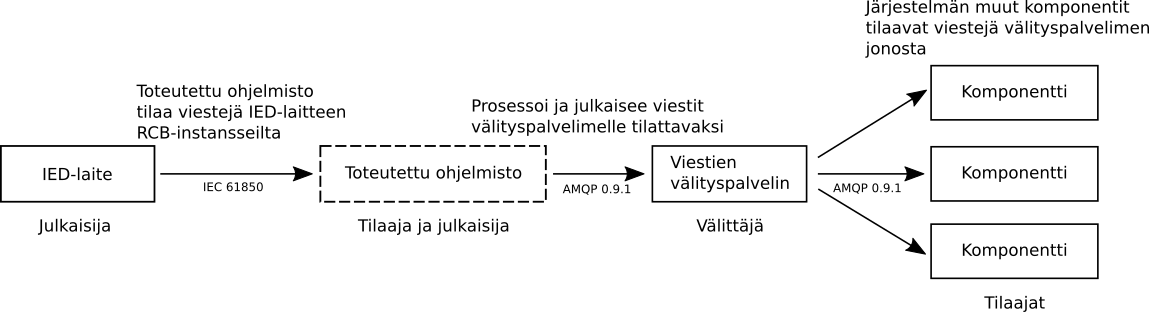
\includegraphics[width=1\textwidth]{pictures/implemented-system-communication.png}
	\caption{Toteutetun ohjelmiston osuus ja rooli kokonaisuudessa tietoliikenteen kannalta.}
	\label{fig:implemented-system-communication}
\end{figure}

Työssä välittäjänä käytettiin \emph{RabbitMQ}-ohjelmistoa \cite{rabbitmq-homepage}, joka on avoimen lähdekoodin välittäjäpalvelin ja perustuu avoimeen \emph{AMQP}-standardiin \cite{amqp-homepage} (engl. \emph{Advanced Message Queuing Protocol}). AMQP määrittää yhteisen protokollan viestintään eri ohjelmistojen välillä verkon yli välityspalvelimen avulla. Verkon ansiosta välityspalvelin voi sijaita eri koneella kuin sitä käyttävät ohjelmistot. Standarista on julkaistu monta eri versiota, ja työn tekohetkellä viimeisin versio oli 1.0. Kuitenkin RabbitMQ-ohjelmisto oli suunniteltu käytettäväksi standardin version 0.9.1 kanssa, ilman asennettuja lisäosia. Versioiden välinen ero oli suuri ja siirto uuteen ei ollut mahdollista, koska standardin versiot eivät olleet keskenään yhteensopivat. RabbitMQ tuki versiota 0.9.1 ja sen kehittäjät mieltävät standardin version 1.0 kokonaan eri protokollaksi \mbox{\cite{RabbitMQ-Compatibility-and-Conformance}}. Kuvassa \ref{fig:implemented-system-communication} on tietoliikenteen kohtiin merkitty mikä standardi vaikuttaa minkäkin osapuolen kommunikointiin. Tässä työssä välityspalvelin ja siihen yhteydessä olevat ohjelmistot käyttävät AMQP-standardista versiota 0.9.1.


\subsection{Advanced Message Queuing -malli ja sen osat}
AMQP-standardi määrittää komponentteja, joiden läpi viestin täytyy kulkea julkaisijalta tilaajalle. Standardissa nämä komponentit määrittää \emph{AMQ-malli} (engl. \emph{AMQ-model}). Kuvassa \ref{fig:amq-model-parts} on esitetty viestin kulku julkaisijalta tilaajalle mallin eri komponenttien läpi. Mallin komponentit ovat \emph{vaihde} (engl. \emph{exchange}), \emph{jono} (engl. \emph{queue}) ja näiden välinen \emph{sidonta} (engl. \emph{binding}). Välityspalvelimen tehtävän voi tiivistää niin, että se ottaa vastaan viestejä julkaisijoilta vaihteeseen. Vaihde reitittää viestejä tilaajille jonoihin määritettyjen sidosten mukaan. Jos tilaaja ei ehdi prosessoida viestejä tarpeeksi nopeasti, palvelin pitää viestit jonossa tilaajalle. Vaihde voi välittää viestin moneen eri jonoon ja yhtä jonoa voi tilata monta eri asiakasta.

\begin{figure}[ht!]
	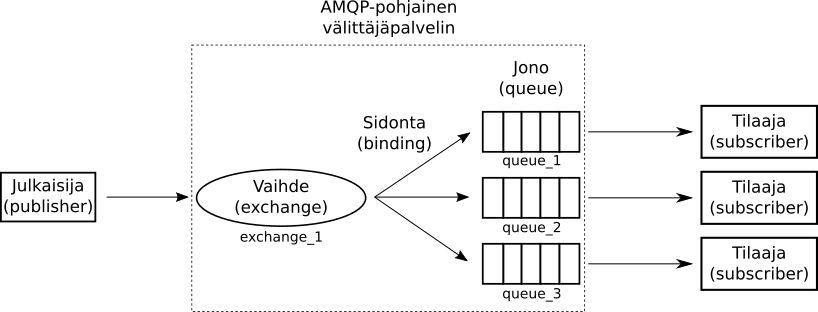
\includegraphics[width=1\textwidth]{pictures/amq-model-parts.png}
	\caption{AMQ-mallin osat ja viestin kulku niiden läpi julkaisijalta tilaajalle (pohjautuu kuvaan \mbox{\cite[s.~11]{AMQP-specification}}).}
	\label{fig:amq-model-parts}
\end{figure}

AMQP on ohjelmoitava protokolla siinä mielessä, että julkaisija ja tilaaja voivat määrittää komponentteja ja reitityksiä palvelimelle verkon yli ajon aikana tarpeidensa mukaan. Välittäjäpalvelin ei määritä kuin oletusvaihteet valmiiksi käytettäväksi. Toisin sanoen julkaisuja voi luoda vaihteita ja tilaaja voi luoda jonoja ja sidoksia vaihteiden ja jonojen välille. Voidaan sanoa että julkaisija ja tilaaja tekevät uusia instansseja AMQ-mallin komponenteista palvelimelle. Vaihteiden ja jonojen instansseilla täytyy olla välityspalvelimella yksilöivät nimet, jokainen nimi asetetaan instanssin luonnin yhteydessä. Esimerkkinä kuvassa \ref{fig:amq-model-parts} on AMQ-mallin komponenttien alla niille määritetyt nimet. Vaihteella on esimerkiksi nimi exchange\_1 ja ylimmällä jonolla queue\_1. Tällä ohjelmoitavalla ominaisuudella välityspalvelin voidaan konfiguroida toteuttamaan erilaisia skenaarioita vapaasti ja se antaa kehittäjille vapautta toteutukseen.


\subsection{Vaihde (exchange) ja reititysavain (routing-key)}
Jotta viesti voidaan kuljettaa välittäjäpalvelimen läpi, täytyy julkaisijan aloittaa määrittämällä käytetty vaihde ja sen tyyppi. Julkaisija voi myös käyttää palvelimen oletusvaihdetta. Vaihde on komponentti, joka ottaa vastaan viestejä ja reitittää niitä jonoihin vaihdetyypin (engl. exchange type) ja sidosten mukaan. Vaihteet eivät ikinä tallenna viestejä. Vaihde voi tiputtaa viestin, jos se ei täsmää minkään määritetyn reitityksen kanssa. AMQ-malli määrittää seuraavat käytettävät vaihdetyypit:
\begin{itemize}
	\item \emph{suoravaihde} (engl. \emph{direct exchange}),
	\item \emph{hajautusvaihde} (engl. \emph{fanout exchange}), ja
	\item \emph{aihepiirivaihde} (engl. \emph{topic exchange}).
\end{itemize}

Näitä tyyppejä ja kuinka ne toimivat käydään tarkemmin läpi tulevissa kappaleissa. Tyypin lisäksi vaihteella on myös attribuutteina \emph{nimi} (engl. \emph{name}), \emph{kestävyys} (engl. \emph{durability}), \emph{automaattinen poisto} (engl. \emph{auto-delete}). Nimi yksilöi vaihteen palvelimella ja tilaaja käyttää tätä nimeä sidoksen tekemiseen jonon ja vaihteen välille. AMPQ-standardissa oletetaan, että nimi on jo tiedossa etukäteen julkaisijalla ja tilaajalla. AMPQ ei tarjoa toiminnallisuutta instanssien nimien noutamiseen. Kestävyys parametrilla julkaisija voi kertoa palvelimelle, että välitäjä säilyttää vaihteen uudelleenkäynnistysten jälkeen. Jos ei, julkaisijan täytyy määrittää vaihde uudelleen käynnistyksen jälkeen. Automaattinen poisto kertoo poistaako välittäjä vaihteen automaattisesti, kun viimeinen siihen sidottu jono on poistettu ja julkaisija ei ole enää yhteydessä.

Kaikki julkaisijan ja tilaajan kutsut välittäjäpalvelimelle, jotka tekevät uuden instanssin komponentista, ovat esitteleviä (engl. declare). Tämä tarkoittaa että palvelin tekee tarvittaessa uuden instanssin komponentista, jos sitä ei ole jo olemassa ja vastaa onnistuneesti molemmissa tapauksissa. Tilanne tulee esimerkiksi silloin kun kaksi julkaisijaa käyttävät samaa vaihdetta keskenään. Toinen ei tiedä onko toinen jo määrittänyt instanssin vaihteesta palvelimelle, esimerkiksi silloin kun ohjelmat käynnistyvät eri aikaan. Jos kummatkin julkaisijat eksplisiittisesti määrittävät saman käytettävän vaihteen. Palvelin vastaa kummallekin onnistuneesti ja tuloksena palvelimella on vain yksi instanssi halutusta vaihteesta. Sama toiminta pätee kaikkiin välittäjäpalvelimen kutsuihin, jotka tekevät uusia instansseja komponenteista.

Vaihde reitittää viestejä jonoihin sen sidosten ja tyypin mukaan. Reititykseen liittyy tärkeä asia, joka on \emph{reititysavain} (engl. \emph{routing-key}). Reititysavain on kuin virtuaalinen osoite viestissä, jonka julkaisija liittää viestiin julkaisun yhteydessä. Tilaaja käyttää myös reititysavainta jonon määrityksen yhteydessä. Vaihde, tyypistä riippuen, voi käyttää tätä avainta reititykseen eri jonoihin. Viestin reititysavainta voi hyvin verrata lähetettävän sähköpostin saaja-kenttään. Saaja kertoo vastaanottajan sähköpostiosoitteen, johon viesti on tarkoitus lähettää. Reititysavain toimii juurikin näin suorassa viestin lähetyksessä, mutta eroaa muissa.


\subsection{Suoravaihde (direct exchange)}
\label{ch:direct-exchange}
Julkaisija voi määrittää vaihteen instanssin tyypiksi suoravaihteen (engl. direct exchange). Suoravaihde reitittää viestin jonoihin vastaavan reititysavaimen perusteella. Suoravaihde reitittää seuraavasti:
\begin{itemize}
	\item tilaaja määrittää sidoksen reititysavaimella K,
	\item julkaisija julkaisee viestin reititysavaimella R,
	\item vaihde välittää viestin jonoon jos K = R,
	\item muuten vaihde tiputtaa tai palauttaa viestin lähettäjälle.
\end{itemize}
Kuvassa \ref{fig:amqp-direct-exchange} on esitetty suoravaihteen toiminta. Vaihteeseen on tehty sidoksia reititysavaimilla error ja info. Yksi tilaaja voi luoda sidoksia samaan vaihteeseen monella eri reititysavaimella. Näin tilaaja voi tilata viestejä mistä on kiinnostunut. Kuvassa \ref{fig:amqp-direct-exchange} julkaisija julkaisee viestin reititysavaimella info. Viesti päätyy molempiin queue\_1 ja queue\_2 jonoon. Reititysavaimella error, viestit päätyvät vain jonoon queue\_1. Välittäjäpalvelin tarjoaa suoravaihteesta oletusvaihteen nimeltä \emph{amq.direct}. \mbox{\cite[s.~27]{AMQP-specification}}

\begin{figure}[ht!]
	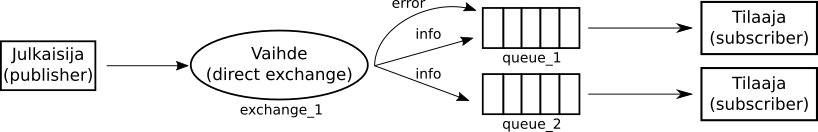
\includegraphics[width=1\textwidth]{pictures/amqp-direct-exchange.png}
	\caption{Suoravaihde (engl. direct exchange), reitittää suoraan sidoksen reititysavaimen mukaan (pohjautuu kuvaan \mbox{\cite{RabbitMQ-Tutorial-Routing}}).}
	\label{fig:amqp-direct-exchange}
\end{figure}


\subsection{Hajautusvaihde (fanout exchange)}
Julkaisija voi määrittää vaihteen instanssiksi hajautusvaihteen (engl. fanout exchange). Hajatusvaihde reitittää viestit kaikkiin sen jonoihin reititysavaimesta välittämättä. Hajautusvaihde toimii seuraavasti:
\begin{itemize}
	\item tilaaja määrittää sidoksen vaihteeseen reititysavaimella K,
	\item julkaisija julkaisee viestin reititysavaimella R,
	\item vaihde välittää viestin kaikkiin siihen sidottuihin jonoihin, reititysavaimesta riippumatta.
\end{itemize}
Kuvassa \ref{fig:amqp-fanout-exchange} on esitetty hajautusvaihteen toiminta. Vaihteeseen exchange\_1 on tehty kolme eri sidosta jonoihin queue\_1, queue\_2 ja queue\_3. Julkaisijan lähettämä viesti lähetetään kaikkiin kolmeen sidottuun jonoon, viestin ja jonojen reititysavaimista riippumatta. Välittäjäpalvelin tarjoaa hajautusvaihteesta oletusvaihteen nimeltä \emph{amq.fanout}. \mbox{\cite[s.~27]{AMQP-specification}}

\begin{figure}[ht!]
	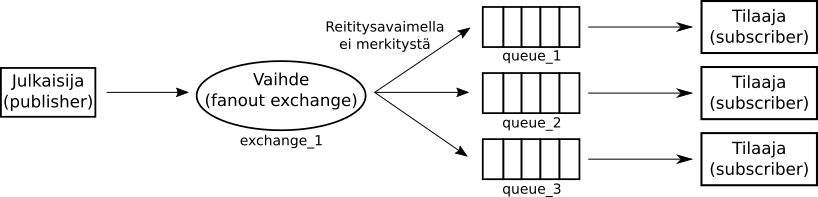
\includegraphics[width=1\textwidth]{pictures/amqp-fanout-exchange.png}
	\caption{Hajautusvaihde (engl. fanout exchange) reitittää kaikkiin siihen sidottuihin jonoihin riippumatta reititysavaimesta (pohjautuu kuvaan \mbox{\cite{RabbitMQ-AMQP-0-9-1-Model-Explained}}).}
	\label{fig:amqp-fanout-exchange}
\end{figure}


\subsection{Aihepiirivaihde (topic exchange)}
Aihepiiri-vaihdetyyppi (engl. topic exchange) reitittää viestejä sidottuihin jonoihin reititysavaimen mukaan kuin suoravaihde, mutta tarjoaa lisäksi sääntöjä monen avaimen samanaikaiseen yhteensopivuuteen. Sidoksen reititysavaimen sijaan voidaan puhua reitityskaavasta (engl. routing pattern). Aihepiiri vaihde toimii seuraavasti:
\begin{itemize}
	\item tilaaja määrittää sidoksen vaihteeseen reitityskaavalla P,
	\item julkaisija julkaisee viestin reititysavaimella R,
	\item vaihde välittää viestin jonoon, jos sen reitityskaava P sopii reititysavaimeen R.
\end{itemize}
Aihepiirivaihteessa reititysavaimen täytyy olla lista sanoja, jotka ovat erotettu pisteillä ja ovat yhdessä maksimissaan 255 merkkiä pitkä \mbox{\cite[s.~35]{AMQP-specification}}. Sanat saavat sisältää kirjaimia A-Z ja a-z, ja numeroita 0-9. Yleensä avaimeen sijoitetaan sanoja mitkä liittyvät viestin sisältöön. Tilaajan määrittämä sidoksen reitityskaava voi olla samaa muotoa kuin reititysavain, mutta sanojen tilalla voidaan käyttää seuraavia erikoismerkkejä:
\begin{itemize}
	\item \textbf{*} (tähti), voi vastata mitä tahansa yhtä sanaa,
	\item \textbf{\#} (risuaita), voi vastata nolla tai monta sanaa. \mbox{\cite[s.~27]{AMQP-specification}}
\end{itemize}

Kuvassa \ref{fig:amqp-topic-exchange} on esitetty aihepiirivaihteen toiminta. Vaihteeseen exchange\_1 on sidottu jono queue\_1 reitityskaavoilla \emph{app1.\#} ja \emph{*.*.warn}. Ja jono queue\_2 reitityskaavalla \emph{*.log.*}. Oletetaan, että julkaisija lähettää viestejä avaimella muodossa \emph{ohjelma.kanava.taso}, jossa \emph{ohjelma} kuvaa julkaisijan nimeä. \emph{Kanava} kuvaa lokitusväylää ja \emph{taso} kuvaa viestin tasoa (warning, error, info jne.). Voisi sanoa että queue\_1 on kiinnostunut kaikista ohjelmalta app1 tulevista viesteistä ja myös kaikista varoitustason (warning) viesteistä. Jono queue\_2 on vain kiinnostunut kaikista log-väylän viesteistä.

\begin{figure}[ht!]
	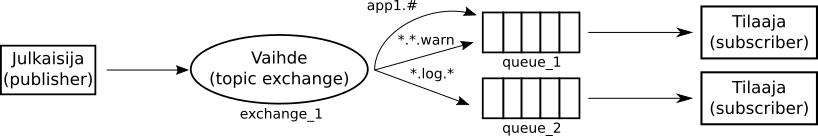
\includegraphics[width=1\textwidth]{pictures/amqp-topic-exchange.png}
	\caption{Aihepiirivaihde (engl. topic exchange), reitittää kaikkiin siihen sidottuihin jonoihin, joiden reitityskaava sopii viestin reititysavaimeen (pohjautuu kuvaan \mbox{\cite{RabbitMQ-Tutorial-Topics}}).}
	\label{fig:amqp-topic-exchange}
\end{figure}

Nyt jos julkaisija lähettää viestin avaimella \emph{app1.debug.warn}, vaihde välittää viestin jonoon queue\_1, mutta ei jonoon queue\_2. Avaimella \emph{app2.log.info} viesti välitetään vain jonoon queue\_2. Avaimella \emph{app1.log.warn} viesti lähetään molempiin jonoihin. Kun taas avaimella \emph{app2.debug.info} viestiä ei lähetetä yhteenkään jonoon.

Aihepiirivaihde on vaihdetyypeistä monimutkaisin, mutta kattaa ison määrän erilaisia käyttötapauksia. Vaihteen avulla tilaajat voivat tilata viestejä, joista ovat esimerkiksi kiinnostuneita. Aihepiirivaihdetta voi käyttää kuin aikaisempia vaihdetyyppejä. Jos jono sidotaan reitityskaavalla \#, se vastaanottaa kaikki viestit kyseiseltä vaihteelta ja käyttäytyy kuin hajautusvaihde. Jos jono sidotaan ilman merkkejä * ja \#, niin se käyttäytyy samalla tavalla kuin suoravaihde. \mbox{\cite{RabbitMQ-Tutorial-Topics}}


\subsection{Jonon määritys ja viestien kuittaaminen}
AMQ-mallissa jono (engl. queue) on vaihteen ja tilaajan välissä oleva puskuri (kuva \ref{fig:amq-model-parts}), joka tallentaa tilaajalle tulevia viestejä. Jono pitää viestejä jonossa tilaajalle, kunnes tämä ehtii prosessoida ne. Yksi jono voi puskuroida viestejä monelle eri tilaajalle. Jotta jonoon saapuu viestejä, täytyy tilaajan sitoa (engl. binding) jono palvelimella olemassa olevaan vaihteeseen. Tällä mekanismilla tilaaja voi valita mistä julkaisijasta on kiinnostunut. Tilaaja voi sitoa saman jonon moneen eri julkaisijaan. Tämä mahdollistaa viestien tilaamisen monelta eri vaihteelta. Sidos vaihteeseen tehdään vaihteen nimellä, eli tilaajan täytyy tietää vaihteen nimi etukäteen. Jonolla tilaaja voi määrittää attribuutteja. Jotkin attribuutit ovat samoja kuin vaihteella. Tilaaja voi määrittää jonolle \emph{nimen} (engl. \emph{name}), \emph{kestävyyden} (engl. \emph{durable}), \emph{poissulkevuuden} (engl. \emph{exclusive}) ja \emph{automaattisen poiston} (engl. \emph{auto-delete}). Nimi yksilöi jonon palvelimella. Tilaaja voi halutessaan pyytää palvelinta generoimaan yksilöivän nimen jonolle automaattisesti. Kestävyys-attribuutti säilyttää jonon palvelimella uudelleenkäynnistyksen jälkeen. Poissulkeva rajoittaa jonon vain yhdelle tilaajalle ja palvelin poistaa jonon kun yhteys tilaajaan katkeaa. Automaattinen poisto poistaa jonon palvelimelta automaattisesti kun yhteys viimeiseen tilaajan on katkennut. \mbox{\cite{RabbitMQ-AMQP-0-9-1-Model-Explained}}

Jos saman nimisen jonoon on liittynyt monta eri tilaajaa. Palvelin lähettää viestin jonosta vain yhdelle tilaajalle kerrallaan kiertovuorottelu (engl. round-robin) periaatteen mukaan. Sama viesti lähetetään ainoastaan toiselle tilaajalle jos se edelleenlähetetään virheen tai peruutuksen seurauksena \mbox{\cite[s.~11--12]{AMQP-specification}}. Tilaajan täytyy määrittää jonolle sen käyttämä viestin kuittaamisen (engl. acknowledge) malli ennen kuin jono poistaa viestin puskurista. Malleja on kaksi:
\begin{itemize}
	\item automaattinen, jolloin palvelin poistaa viestin jonosta heti kun se on lähetetty tilaajalle,
	\item eksplisiittinen, jolloin palvelin poistaa viestin, kun tilaaja on lähettänyt kuittauksen palvelimelle.
\end{itemize}
Tilaaja voi lähettää viestistä kuittauksen milloin vain prosessoinnin aikana. Heti kun viesti on vastaanotettu tai silloin kun viesti on prosessoitu. \mbox{\cite[s.~29]{AMQP-specification}}